\chapter{Radio electronic characteristics}

By the time the \gls{rf} signal has reached the acoustic transducer, it has
been synthesized from a reference signal, amplified, and matched to the
impedance of the \gls{aod} transducer. We are going to inspect the \gls{rf}
signal characteristics at each transmission and find that each stage
unintentionally carries out frequency dependent amplitude modulation which,
as we will see in the next chapter, is responsible for the complex intensity
distribution observed with the photodiode.

\section{Digital signal synthesizer}

We already covered the fundamental functionality of the \gls{dds} in XX and
its integration in our experimental setup in YY. In this section we want to
check up on the suspected characteristics disclosed in these sections through
real world measurements.

\subsection{Discrete frequency spectrum}

\begin{figure}[h]
  \centering
  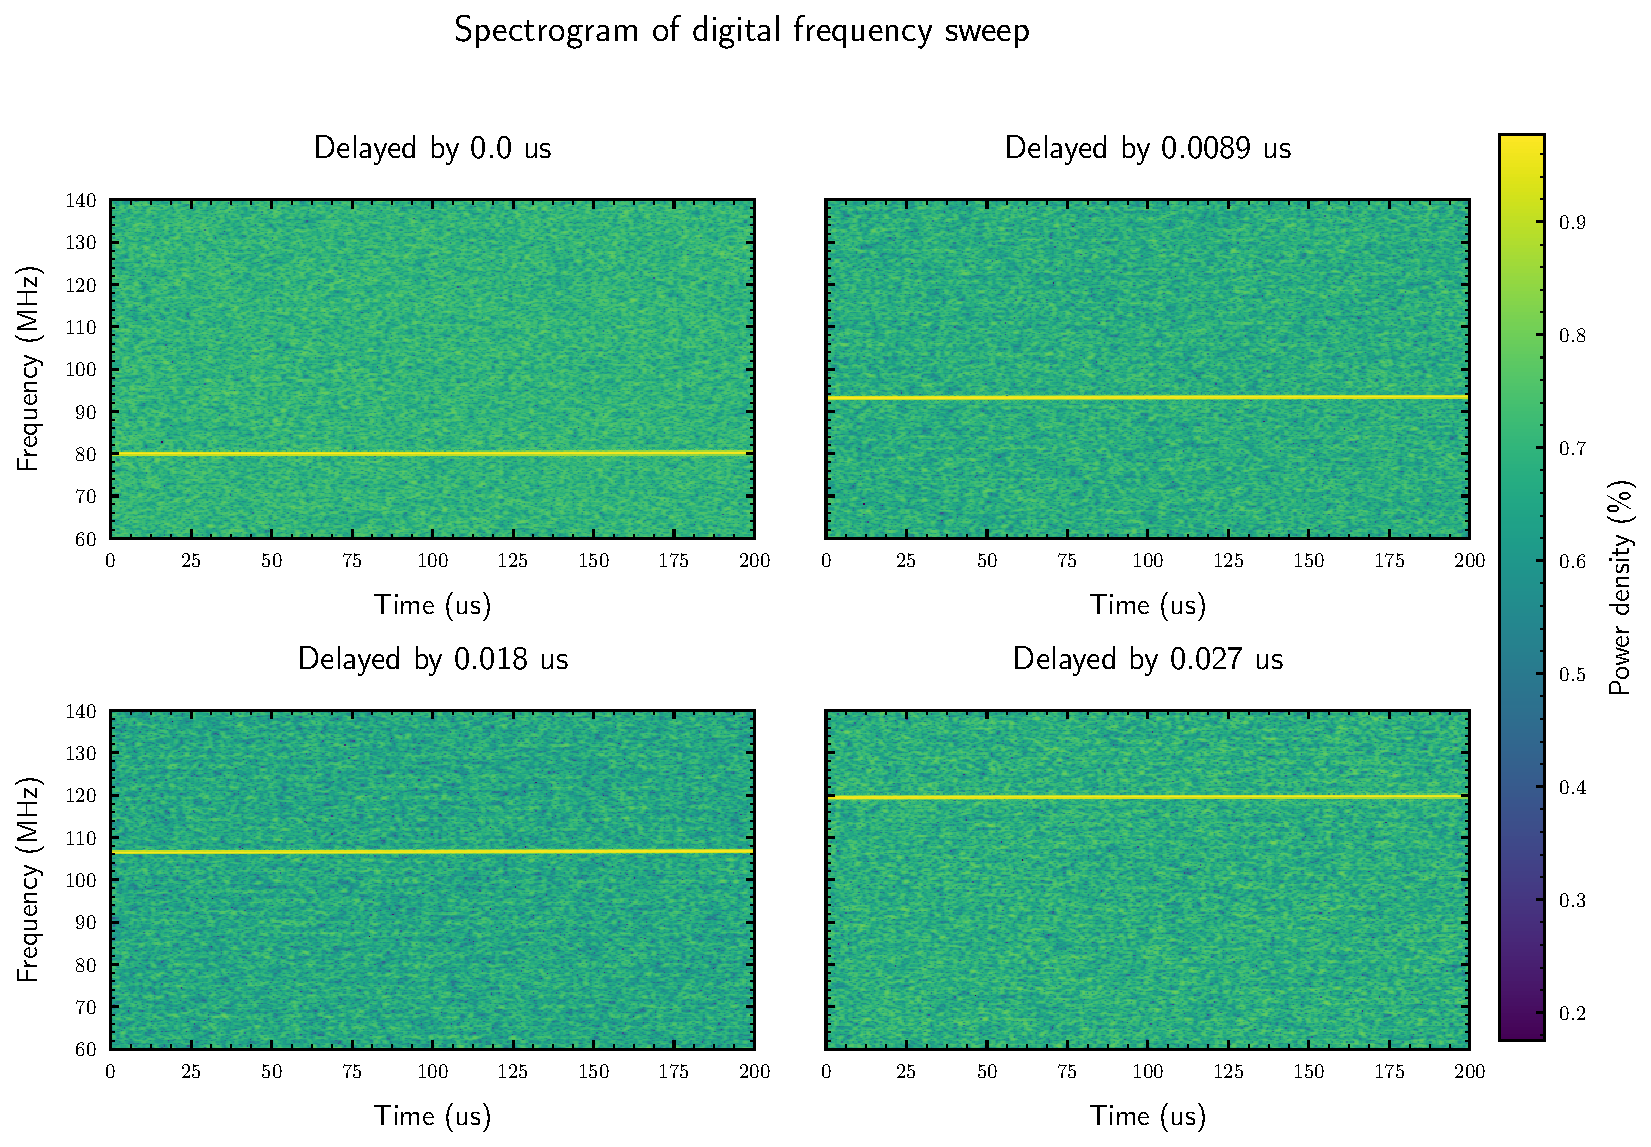
\includegraphics[width=\textwidth]{\figuredir{signal/synthesis/spectrogram.pdf}}
  \captionsetup{width=.8\textwidth}
  \caption{Spectrogram of delayed time windows of the \gls{dds} output signal
    configured to perform a frequency sweep from \SI{80}{\mega\hertz} to
    \SI{120}{\mega\hertz}. For an ideal linear sweep we would expect a linear
    timeline of the frequency, instead we observe a discrete set of
    frequencies which reflects the digital nature of the \gls{dds}.}
  \label{fig:signal_synthesis_spectrogram}
\end{figure}

\subsection{Amplitude frequency response}

\section{Amplifier}

\subsection{Transmission spectrum}

\subsection{Amplitude frequency response}

\section{Acoustic transducer}

\subsection{Reflection spectrum}
